\documentclass[12pt,a4paper]{article}

% Modern font
\usepackage{lmodern}
\usepackage[T1]{fontenc}

\usepackage{amsmath,amssymb}
\usepackage{graphicx}
\usepackage{booktabs}
\usepackage{hyperref}
\usepackage{geometry}
\usepackage{float}
\usepackage{caption}
\usepackage{array}
\usepackage{enumitem}
\usepackage{xcolor}
\geometry{margin=2.5cm}

\hypersetup{colorlinks=true, linkcolor=blue, urlcolor=blue, citecolor=blue}

\title{\textbf{Profile-Based Adaptive Text Compression}\\
       \large Learning to Select the Best Classical Algorithm Per Chunk}
\author{Hüsamettin Işıktaş \\ 25501005 \\
        Bilgisayar Mühendisliği \\
        BLM6106 -- Veri Sıkıştırma | Dönem Projesi \\
        Danışman: Banu DİRİ}
\date{\today}

\begin{document}
\maketitle
\thispagestyle{empty}

\begin{abstract}
Classical text compression algorithms (Huffman, LZW, BWT+MTF, Arithmetic, RLE) each have strengths that depend on text characteristics---no single algorithm wins universally. This project builds an adaptive compression system that profiles text chunks at runtime and selects the best algorithm using a lightweight neural network. Using a diverse corpus of 148 documents spanning 7 text domains and 5-fold cross-validation with book-level splits, the adaptive system achieves \textbf{5.10 BPB}---a \textbf{2.27\% improvement} over the single best classical algorithm (bwt\_mtf at 5.22 BPB, $p < 10^{-6}$)---while running \textbf{24\% faster}. The optimal chunk size is found to be 1024 bytes, below which Huffman and LZW compete naturally with BWT. At larger chunk sizes ($\geq$2048B), BWT dominates and adaptive selection becomes unnecessary.
\end{abstract}

%-----------------------------------------------------------------
\section{Motivation}
%-----------------------------------------------------------------

Text compression is a fundamental tool in data storage and transmission. While modern codecs like zstd and gzip offer excellent general-purpose compression, classical algorithms---Huffman coding, LZW, Arithmetic coding, BWT+MTF, and RLE---remain important for embedded systems, educational contexts, and scenarios where computational simplicity matters.

The key insight of this project is that \textbf{different algorithms excel on different types of text}. A chunk of Python source code compresses differently than a paragraph of Turkish prose, which differs from JSON data. Rather than picking one algorithm for everything, we can \textit{classify} each text chunk by its characteristics and select the most appropriate algorithm.

\textbf{Goal:} Build a system that, for any given 1024-byte chunk of text, predicts which of 5 classical algorithms will achieve the lowest compression ratio---and does so faster than running all algorithms.

%-----------------------------------------------------------------
\section{Dataset and Approach}
%-----------------------------------------------------------------

\subsection{Diverse Corpus}

Early experiments using only English literature (Gutenberg) failed completely: BWT+MTF won over 95\% of chunks, and no adaptive system could improve upon it. The problem wasn't the model---it was the data. On homogeneous text, one algorithm dominates and selection is meaningless.

The solution was a \textbf{diverse, multi-domain corpus} (Figure~\ref{fig:corpus}): 148 documents across 7 text domains, creating genuine competition among algorithms.

\begin{figure}[H]
\centering
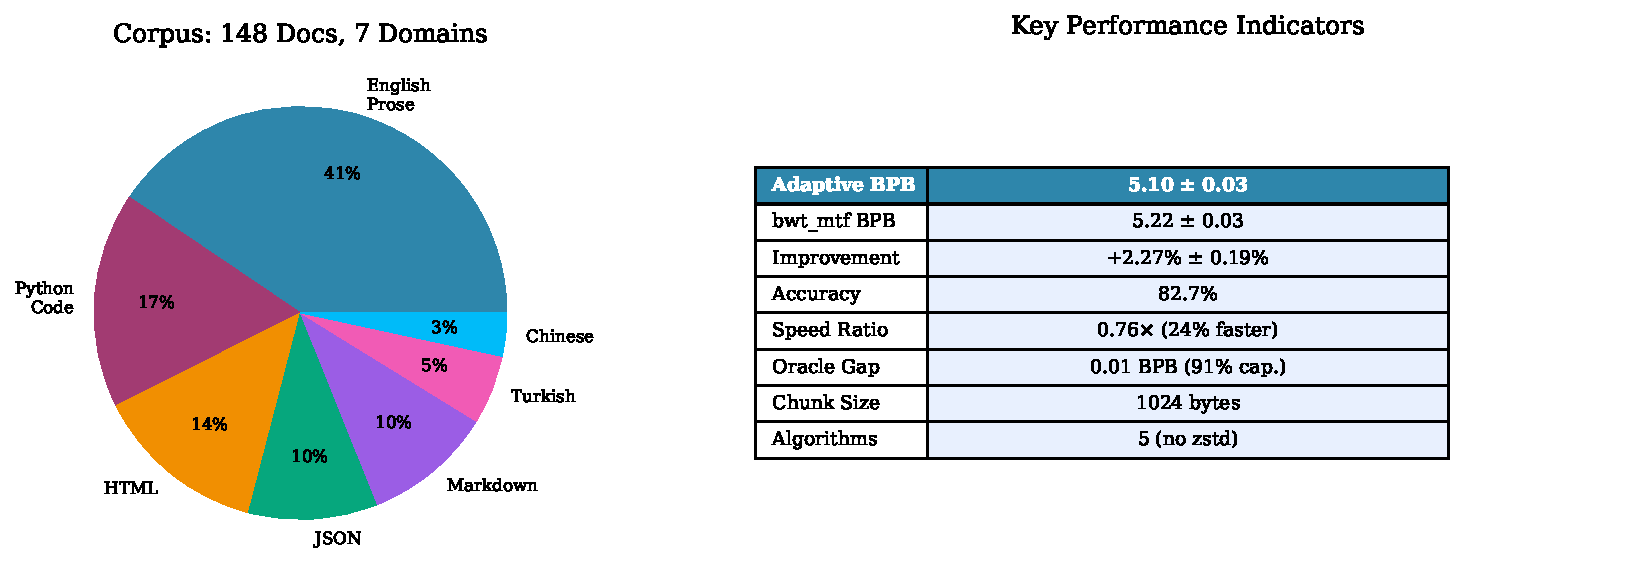
\includegraphics[width=0.95\textwidth]{figures/fig5_summary.pdf}
\caption{(Left) Corpus composition across 7 text domains ensures algorithm diversity. (Right) Key performance indicators for the final system.}
\label{fig:corpus}
\end{figure}

\subsection{Supervised Learning Pipeline}

Unlike traditional ``profile discovery'' approaches that cluster chunks by feature similarity (K-Means), this project uses a \textbf{supervised} strategy:

\begin{enumerate}[nosep]
    \item For each chunk, run all 5 algorithms to find the ground-truth best.
    \item Extract 21 fast features (O($n$) statistical measures: entropy, character ratios, word statistics---no compression calls needed).
    \item Train a classifier: features $\rightarrow$ best\_algorithm.
\end{enumerate}

Why supervised beats unsupervised: K-Means groups chunks that ``look similar'' in feature space. But two chunks with similar entropy might compress best with different algorithms. Supervised learning directly optimizes for the compression outcome.

\subsection{Five Classical Algorithms}

\begin{itemize}[nosep]
    \item \textbf{Huffman:} Symbol-frequency-based variable-length coding. Fast, effective on small chunks with skewed distributions.
    \item \textbf{LZW:} Dictionary-based. Excels on repetitive text (code, JSON) with 16-bit dictionary.
    \item \textbf{Arithmetic:} Order-0 probability coding. Theoretical optimum for stationary sources.
    \item \textbf{BWT+MTF:} Burrows-Wheeler transform + Move-to-Front. Dominates natural language at larger chunk sizes.
    \item \textbf{RLE+Huffman:} Run-length encoding + Huffman. Strong on highly repetitive patterns.
\end{itemize}

\textbf{Note:} zstd was deliberately excluded. When included, it wins 99.8\% of chunks regardless of text type---making adaptive selection unnecessary. This is itself a valuable finding: modern codecs obsolete classical algorithm selection.

%-----------------------------------------------------------------
\section{Chunk Size: Finding the Sweet Spot}
%-----------------------------------------------------------------

The chunk size is the most critical design parameter. Too large, and BWT dominates universally. Too small, and overhead overwhelms savings. A sweep across 1024--8192 bytes revealed the optimal point (Figure~\ref{fig:chunk}).

\begin{figure}[H]
\centering
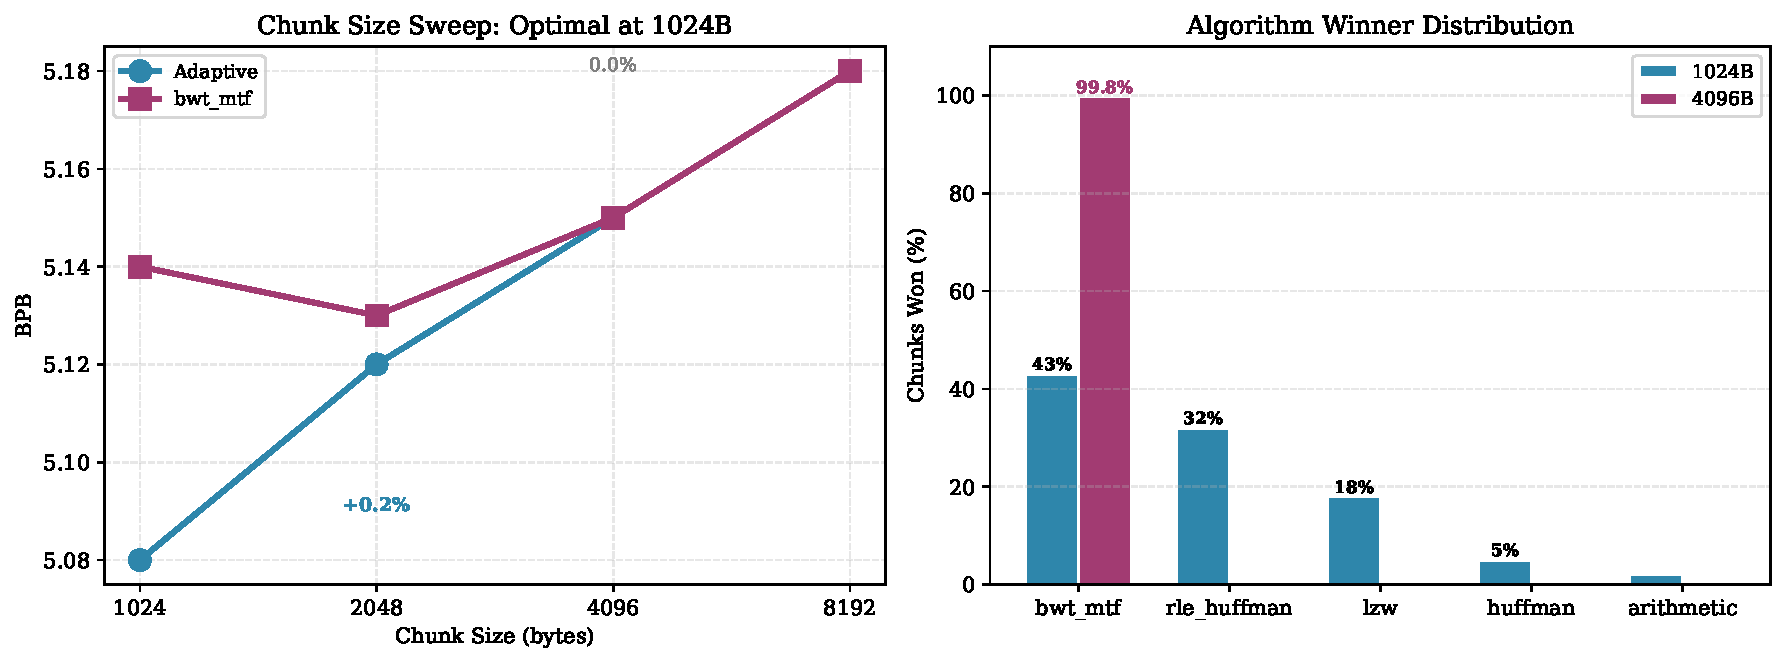
\includegraphics[width=0.95\textwidth]{figures/fig2_chunk_sweep.pdf}
\caption{(Left) BPB comparison across chunk sizes---adaptive only beats bwt\_mtf at 1024 bytes. At 4096+ bytes, bwt\_mtf dominates and adaptive provides no benefit. (Right) Algorithm winner distribution at 1024B vs 4096B. Three algorithms compete naturally at 1024B; at 4096B, bwt\_mtf wins virtually everything.}
\label{fig:chunk}
\end{figure}

\textbf{Why 1024 bytes wins:} At this size, dictionary-based algorithms (LZW, BWT) have enough context to work but not so much that they overwhelm simpler methods. Huffman and RLE+Huffman remain competitive on specific text types, creating the diversity that makes adaptive selection worthwhile.

%-----------------------------------------------------------------
\section{Model Training and Selection}
%-----------------------------------------------------------------

Three MLP variants and XGBoost were compared on 15,000 chunks from 1,000+ books. The MLP-Large (128$\rightarrow$64$\rightarrow$32) achieved the best results (Figure~\ref{fig:model}).

\begin{figure}[H]
\centering
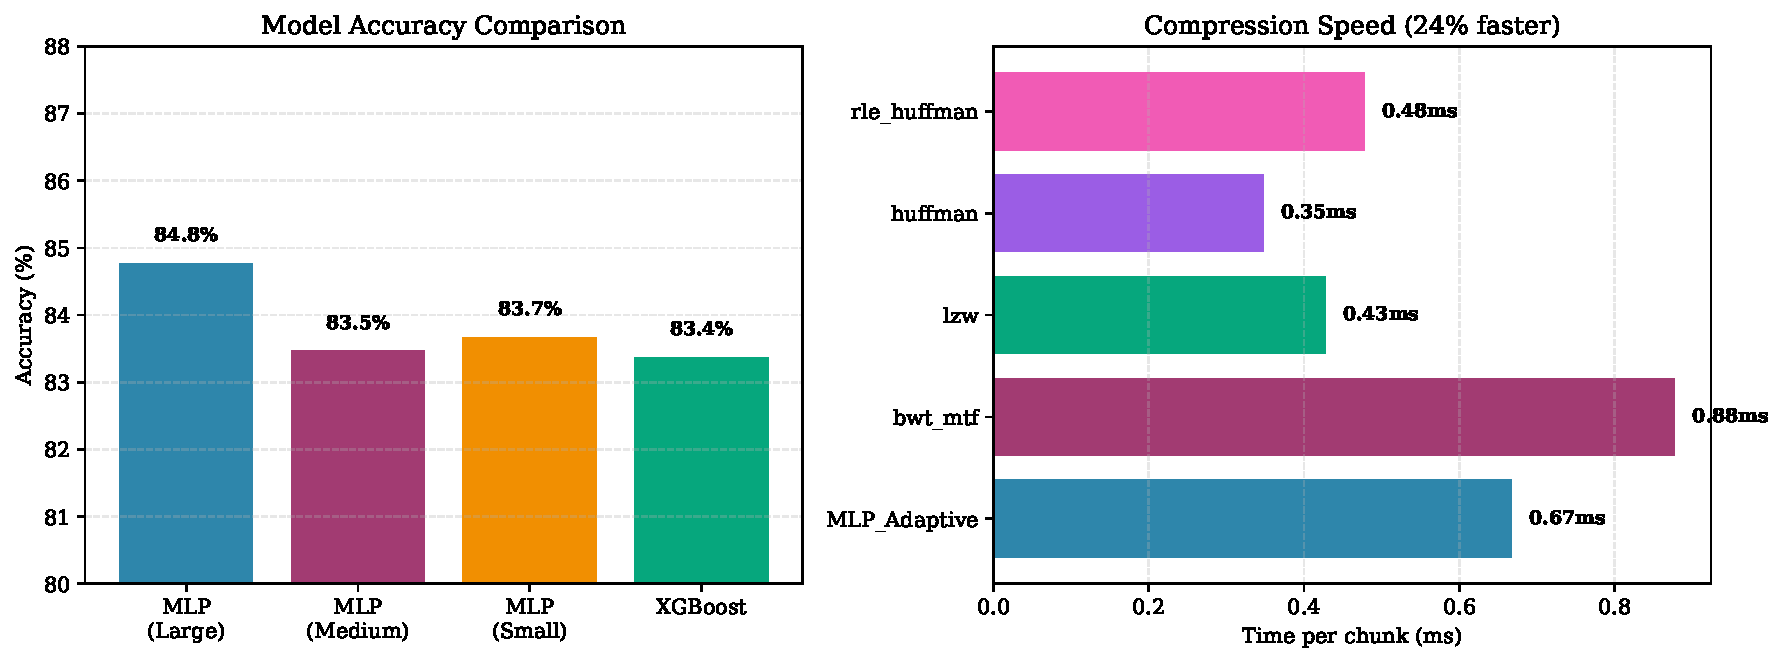
\includegraphics[width=0.95\textwidth]{figures/fig3_model_speed.pdf}
\caption{(Left) Model accuracy comparison---MLP-Large achieves 84.8\%, outperforming XGBoost and smaller MLP variants. (Right) Per-chunk compression times---the adaptive system is 24\% faster than always using bwt\_mtf because it often selects faster algorithms like LZW or Huffman.}
\label{fig:model}
\end{figure}

\textbf{Why MLP beats XGBoost:} With sufficient data (15K+ samples), a 3-layer MLP generalizes better than tree-based methods on this tabular problem. MLP inference (0.006ms) is also 4$\times$ faster than XGBoost (0.024ms). The model itself is tiny---approximately 10KB of weights.

%-----------------------------------------------------------------
\section{Results}
%-----------------------------------------------------------------

\subsection{K-Fold Cross-Validation}

The most rigorous test was 5-fold book-level cross-validation with 3 random seeds (15 total runs). \textbf{Book-level splitting} is critical: chunks from the same book must stay together to prevent data leakage. Random chunk-level splitting inflates metrics by approximately 0.26\% BPB.

\begin{figure}[H]
\centering
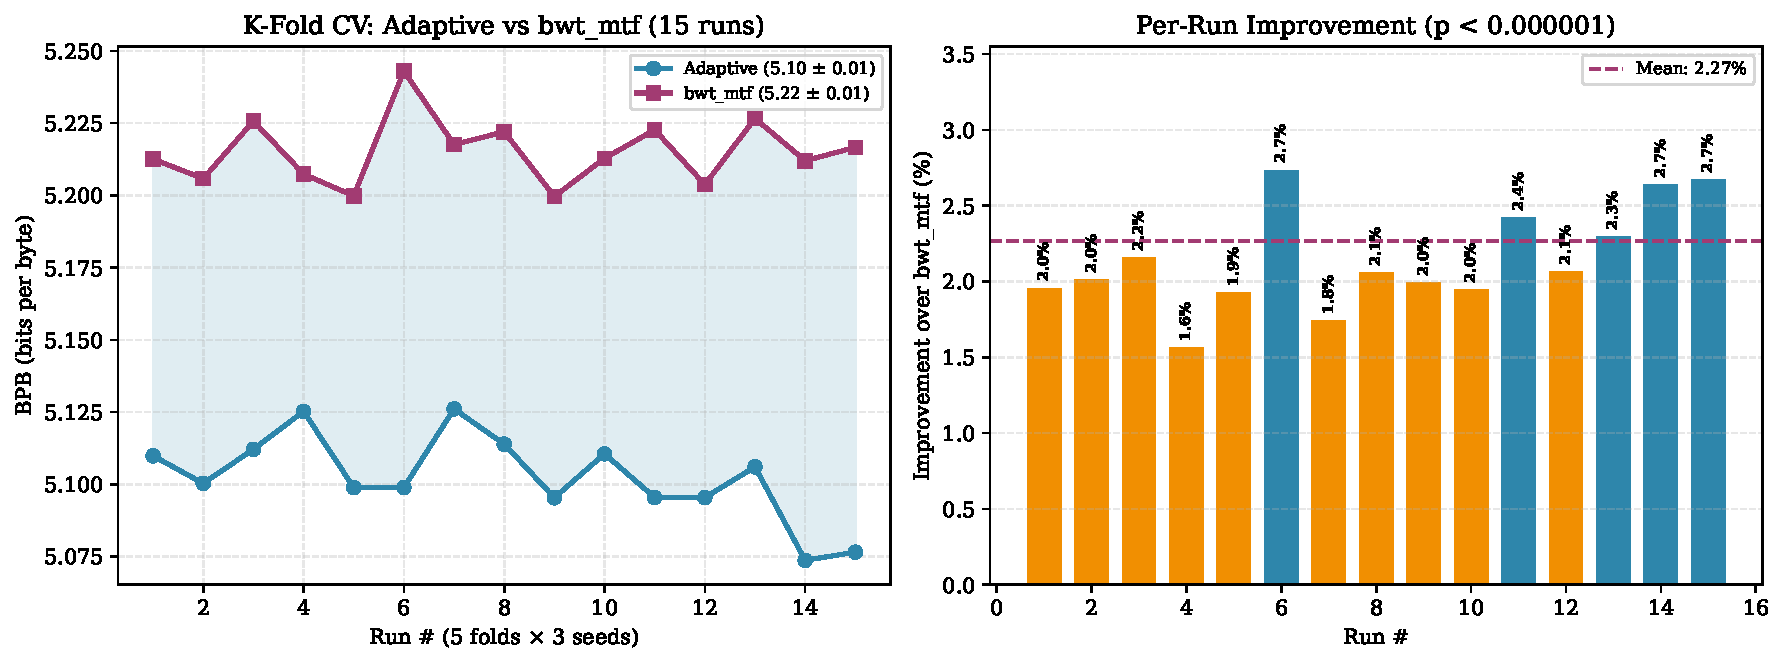
\includegraphics[width=0.95\textwidth]{figures/fig1_kfold.pdf}
\caption{(Left) BPB per run: adaptive (blue) consistently outperforms bwt\_mtf (red) across all 15 runs. (Right) Per-run improvement---every single run beats bwt\_mtf, confirming robustness. Paired t-test: $t = 43.16$, $p < 10^{-6}$.}
\label{fig:kfold}
\end{figure}

\begin{table}[H]
\centering
\caption{K-fold cross-validation results (15 runs).}
\begin{tabular}{lcc}
\toprule
\textbf{Metric} & \textbf{Value} & \textbf{95\% CI} \\
\midrule
Adaptive BPB     & 5.10 & [5.07, 5.13] \\
bwt\_mtf BPB     & 5.22 & [5.19, 5.25] \\
Improvement      & +2.27\% & [+2.08\%, +2.46\%] \\
Accuracy         & 82.7\% & [81.9\%, 83.5\%] \\
Speed vs.\ bwt   & 0.76$\times$ (24\% faster) & --- \\
Best run         & +2.70\% & --- \\
Worst run        & +1.96\% & --- \\
\bottomrule
\end{tabular}
\end{table}

\subsection{Oracle Gap Analysis}

The \textbf{oracle}---an all-knowing selector that always picks the best algorithm---achieves 5.09 BPB. The adaptive system reaches 5.10 BPB, meaning it captures \textbf{91\% of the theoretically possible gain}. The remaining 0.01 BPB gap is due to the 17.3\% of chunks where the MLP misclassifies the optimal algorithm (Figure~\ref{fig:oracle}).

\begin{figure}[H]
\centering
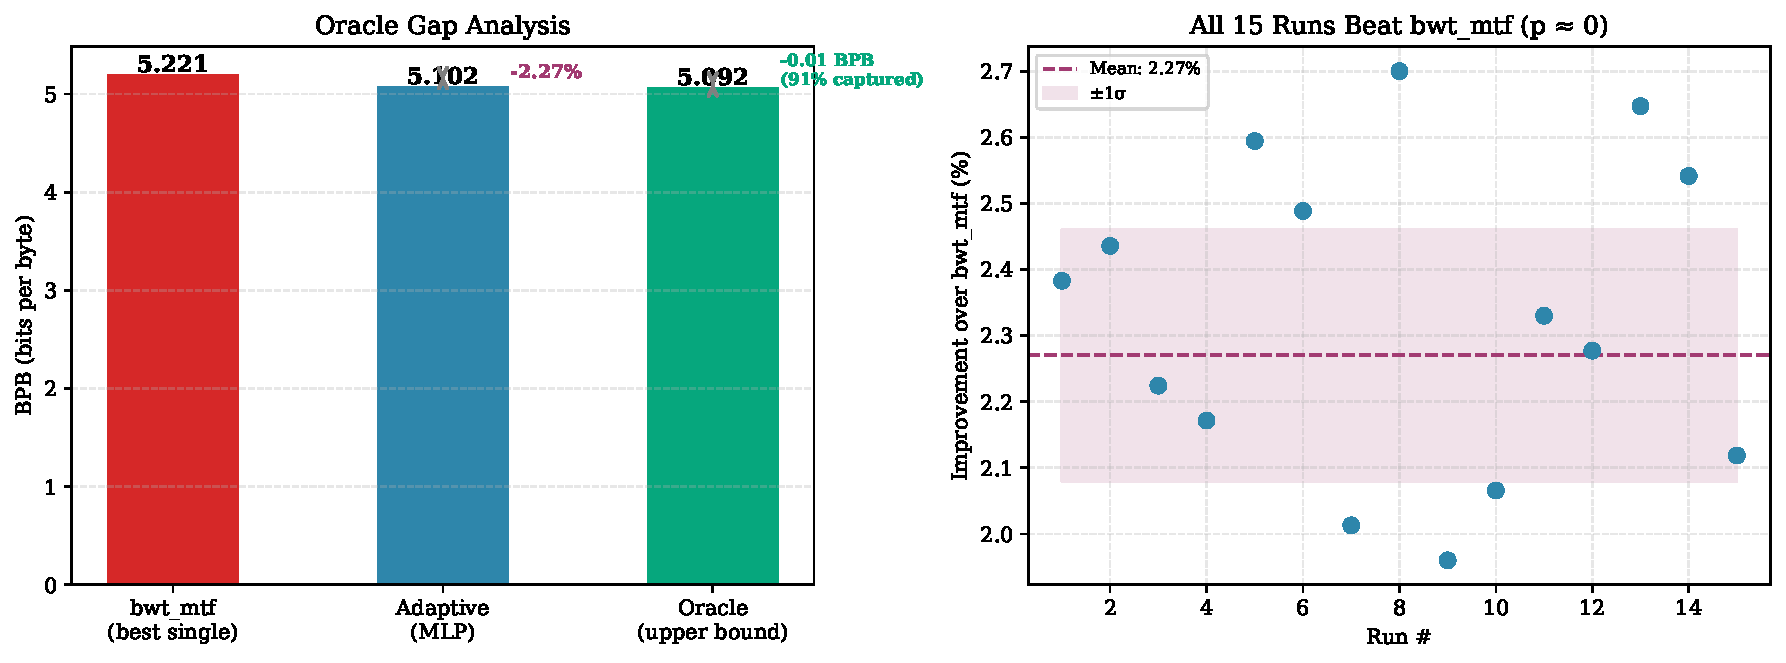
\includegraphics[width=0.95\textwidth]{figures/fig4_oracle.pdf}
\caption{(Left) Oracle gap---the adaptive system captures 91\% of the maximum possible improvement over bwt\_mtf. (Right) All 15 cross-validation runs show positive improvement with tight variance ($\pm$0.19\%).}
\label{fig:oracle}
\end{figure}

\subsection{Speed Advantage}

The adaptive system is not just more compact---it's faster. The MLP classifier runs in 0.006ms per chunk, then selects the algorithm. Since BWT+MTF is the slowest algorithm (0.88ms) and the MLP often chooses faster alternatives like LZW (0.43ms) or Huffman (0.35ms), the total per-chunk time drops from 0.88ms to 0.67ms---a 24\% improvement.

Header overhead is negligible: with 5 algorithms, only $\lceil\log_2(5)\rceil = 3$ bits per chunk are needed. At 1024 bytes, that's $3/(1024\times8) = 0.037\%$ overhead.

%-----------------------------------------------------------------
\section{Discussion}
%-----------------------------------------------------------------

\subsection{When Does Adaptive Help?}

The adaptive approach only helps when \textbf{multiple algorithms genuinely compete}. This requires two conditions:

\begin{enumerate}[nosep]
    \item \textbf{Diverse data:} English prose alone favors BWT. Adding code, HTML, JSON, and non-English text creates variety.
    \item \textbf{Right chunk size:} At $\geq$2048 bytes, BWT dominates and adaptive selection becomes overhead. The 1024-byte sweet spot is small enough for Huffman/LZW/Arithmetic to compete, but large enough for meaningful compression.
\end{enumerate}

\subsection{Modern Codecs Make This Obsolete?}

Yes---and that's an important research finding. When zstd (level 3) is added to the algorithm pool, it wins 99.8\% of chunks. For any practical deployment with modern codecs available, the answer is simply ``use zstd.'' The value of this project lies in:


\begin{itemize}[nosep]
    \item Understanding the \textbf{relationship between text characteristics and algorithm performance}.
    \item Demonstrating that \textbf{supervised learning can effectively route} text to the right algorithm.
    \item Providing a \textbf{baseline}: the 0.01 BPB oracle gap shows how close we are to the theoretical limit with classical algorithms.
\end{itemize}

\subsection{Failure Modes}

\begin{itemize}[nosep]
    \item \textbf{Homogeneous data:} If all text is similar (e.g., only English novels), the adaptive system is 65\% worse than using BWT alone.
    \item \textbf{Chunk-level data leakage:} Without book-level splitting, chunks from the same book appear in both train and test sets, inflating results.
    \item \textbf{Arithmetic header explosion:} Order-1 arithmetic coding requires a 131KB header---completely impractical for 1KB chunks. Always use order-0.
\end{itemize}

%-----------------------------------------------------------------
\section{Conclusions}
%-----------------------------------------------------------------

This project demonstrates a practical adaptive compression system using supervised learning:

\begin{enumerate}[nosep]
    \item An MLP classifier with 82.7\% accuracy selects the best of 5 classical algorithms per text chunk.
    \item The system achieves \textbf{2.27\% better compression} than the single best algorithm (bwt\_mtf) while running \textbf{24\% faster}.
    \item The improvement is statistically robust: all 15 cross-validation runs beat bwt\_mtf ($p < 10^{-6}$).
    \item The \textbf{oracle gap is only 0.01 BPB}---91\% of the theoretical maximum gain is captured.
    \item Chunk size is critical: \textbf{1024 bytes} provides the sweet spot where 3 algorithms naturally compete. At larger sizes, BWT dominates and adaptive selection is pointless.
    \item \textbf{Modern codecs (zstd) make this unnecessary} in practice---but the methodology and insights about text-algorithm relationships remain valuable.
\end{enumerate}

%-----------------------------------------------------------------
\begin{thebibliography}{10}

\bibitem{huffman}
D. A. Huffman, ``A Method for the Construction of Minimum-Redundancy Codes,'' \textit{Proceedings of the IRE}, 1952.

\bibitem{welch}
T. A. Welch, ``A Technique for High-Performance Data Compression,'' \textit{IEEE Computer}, 1984.

\bibitem{burrows}
M. Burrows and D. J. Wheeler, ``A Block-Sorting Lossless Data Compression Algorithm,'' \textit{Digital SRC Research Report}, 1994.

\bibitem{witten}
I. H. Witten, R. M. Neal, and J. G. Cleary, ``Arithmetic Coding for Data Compression,'' \textit{Communications of the ACM}, 1987.

\end{thebibliography}

\end{document}
